\chapter{Complex Analysis}
\label{chap:complex-analysis}

Complex analysis is the branch of math that deals with calculus for complex functions. It's status as an upper level undergraduate class for majors---often not even taught to physicists---gives the subject a forboding field. But in fact it is much more intuitive than it's cousin real analysis (calculus for real functions) and is quite similar to the vector calculus most first-year physics majors learned. It's techniques, particularly the Residue theorem, are very important in QFT, so we provide a summary of them.

We restrict ourselves to a subclass of complex functions called \emphi{analytic} or sometimes \emphi{holomorphic} functions. These functions are continuous and infinitely differentiable functions of a single complex variable $z$. Uses of the complex conjugate of $z$ are forbidden. Examples of \textit{non}-analytic functions are 
$$z^*z,\qquad |z|,\qquad \mathrm{piecewise\ functions}.$$
We can express this requirement of analyticity in another way: if we write a complex number $z=a+bi$ as a vector $\bm z = (a, -b)^T$, then a complex function $f(z)$ being analytic is equivalent to the vector function $\bm f(\bm z)$ being curl-free and divergence-free in the vector calculus sense:
\begin{e}
  \nabla \cdot \bm f = 0\qquad \nabla \times \bm f = 0.
  \label{eqn:analytic-definition}
\end{e}

Holomorphic functions obey several very useful theorems concerning power series (section \ref{sec:ca-series}) and integration (section \ref{sec:ca-residue}) discussed next.

\section{Series, Poles, and Branch Cuts}
\label{sec:ca-series}

The constraint for analyticity (\ref{eqn:analytic-definition}) seems strict, but most functions in physics nevertheless satisfy it. Polynomials, rational functions, and exponents are all analytic functions. In fact, any function with a Taylor series is analytic. Likewise, analytic functions can be written as a Taylor series which converges in some disk of radius $R$ centered on $z_0$:
\begin{e}
  f(z) = \sum_{n=0}^\infty \frac{(z-z_0)^n}{n!}\eval{\frac{d^n f}{d z^n}}_{z=z_0} \mathrm{\ converges\ for\ all\ }|z-z_0| < R.
  \label{eqn:analytic-taylor-series}
\end{e}
This statement has an immediate consequence, which is that if you know the value of $f(z)$ in a small region---but one big enough to compute all the derivatives of $f$ there---then (\ref{eqn:analytic-taylor-series}) tells you the value of $f$ everywhere in the much larger disk of convergence. In this sense, analytic functions are \emph{unique}.

In some functions (called \emphi{entire} functions), that disk is the entire complex plane, but for most functions the disk can only grow so large before the series diverges. The maximum radius of the disk, called the \emphi{radius of convergence} $R$, is always the distance to the nearest singularity of the function.

A \emphi{singularity} is a location where the function is undefined. The most common singularity is a \emphi{pole}, where $f$ blows up due to dividing by a small number. For example, the function $f(z)=1/z$ has a pole at $z=0$. $1/z^2$ also has a pole at zero, but we would call this a pole of multiplicity two due to the square in the denominator.

The relationship between series and poles is very useful, and sheds light on why some Taylor series of real functions diverge. For example, the function
\begin{e}
  f(x) = \frac{1}{x^2+1}
  \label{eqn:divergence-example}
\end{e}
is defined for all real $x$, and has a seemingly innocent Taylor series
\begin{e}
  \frac{1}{x^2+1} = \sum_{n=0}^\infty (-1)^n x^{2n}.
\end{e}
But try plugging in $x>1$ or $x < -1$ and the Taylor series diverges. That is, it has a radius of convergence 1. We can see why by returning to the original function (\ref{eqn:divergence-example}) and promoting $x$ to a complex variable $z$. Then $f(z)$ has poles at $z=\pm i$, since $1/(i^2+1)$ diverges. The distance between the center of the Taylor series ($0$) and the pole ($i$) is one, so $R=1$.

Luckily, a series diverging is often fixable. Consider $f(z) = \ln{z}$, defined as the function such that $e^{f(z)} = z$. This function has a pole at $z=0$, since $e^{-\infty} = 0$. For this reason, the Taylor series around $z_0=1$ has a radius of convergence of $R=1$, which you can verify for yourself by looking at the series' terms
\begin{e}
  \ln(z) = (z-1)-\frac{(z-1)^2}{2}+\frac{(z-1)^3}{3}-\frac{(z-1)^4}{4}+\dots - (-1)^n\frac{(z-1)^n}{n}.
  \label{eqn:log-expansion-0}
\end{e}
However, we can extend the domain of this function by evaluating the series at a new point, such as $z_1 = (1 + i)/\sqrt{2}$. Since $z_1$ is well within the radius of convergence of (\ref{eqn:log-expansion-0}), we can also find all the derivatives of $\ln(z_1)$ and write out the Taylor series:
\begin{e}
  \ln(z) = \sum_{n=0}^\infty a_n (z-z_1)^n
  \label{eqn:log-expansion-1}
\end{e}
where $a_n$ are new complex constants. Since the only pole of the logarithm is at $z=0$, this series still has a radius of convergence of 1. Since $|i - z_1| < 1$, we can use it to define the logarithm of $i$, which turns out to be $\ln i = i\pi / 2$.

The point is that while $i$ is within the radius of convergence of (\ref{eqn:log-expansion-1}), it is outside the radius of convergence of the original series because $|i-1|>1$. So by introducing the intermediate series centered on $z_1$, we have managed to beat the radius of convergence and define $\ln i$! If we wished, we could go farther and define $\ln z$ at any point in the complex plane (except $z=0$) despite the pole, simply by introducing $z_2$, $z_3$, etc. and walking the radius of convergence of the series over to $z$.\footnote{Note that we do not have a single Taylor series which works for every point; you must chose the right Taylor series which is centered on a nearby point.} This process is called \emphi{analytic continuation} and can be performed on any analytic function. A diagram is given in Figure \ref{fig:ln-analytic-continuation}.

\begin{figure}
  \centering
  \begin{tikzpicture}[scale=1.3]
    \draw (0,-3) -- (0,3);
    \draw (-3,0) -- (3,0);
    \draw [thick] (0.707,0.707) circle (1);
    \filldraw [black] (1,0) circle (2pt) node[anchor=south]{$1$};
    \filldraw [black] (0.707,0.707) circle (2pt) node[anchor=south west]{$z_1$};
    \filldraw [black] (0,1) circle (2pt) node[anchor=west]{$i$};
    \draw [gray] (0.707,-0.707) circle (1);
    \draw [gray] (0,-1) circle (1);
    \draw [gray] (-0.707,-0.707) circle (1);
    \draw [gray] (-1,0) circle (1);
    \draw [gray] (-0.707,0.707) circle (1);
    \node [black] (0,0) {$\mathbf{\times}$};
    \path [draw=black,snake it](-3,0) -- (0,0);
  \end{tikzpicture}
  \caption{Black: The analytic continuation that gives $\ln i = \pi i / 2$ via a Taylor series centered on $z_1$. Gray: the contradicting path giving $\ln i = -3\pi i / 2$, and the wavy line is the branch cut preventing it. The cross in the center is the pole.}
  \label{fig:ln-analytic-continuation}
\end{figure}

Qualitatively speaking, we've shown that the divergence of (\ref{eqn:log-expansion-0}) was a red herring except at $z=0$. The function was perfectly well defined.

Or was it? There is still one property left to check: does the value we got for $\ln i$ depend on the value we chose for $z_1$? At first it seems like the answer is no because the disk of radius $1$ surrounding $z_1$ directly connects $i$ to 1, and the logarithm must be unique in this disk as we discussed just after (\ref{eqn:analytic-taylor-series}).

But there's a flaw in this argument. What if we didn't connect 1 to $i$ directly? We could instead define $z_1 = (1 - i)/\sqrt{2}$, $z_2 = -i$ and so forth, making a series of disks wrapping clockwise around the origin instead of counterclockwise. Try this, and we would get $\ln i = -3\pi i / 2$ instead.\footnote{In the case of the logarithm, it is simple to find the $2\pi$ offset which analytic continuation produces. It happens that $\ln(re^{i\theta})$, where $r$ and $\theta$ are real, is $\ln r + i\theta$. Check this by exponentiating $\ln r + i\theta$ and confirming it is equal to $re^{i\theta}$. Then defining $z_i$ along a circle of radius $r=1$ keeps increasing the imaginary component of $z_i$ as $\theta$ is increased until the circle is complete and the analytic continuation has accumulated a $2\pi i$ offset.}

But it cannot be that $\ln i = \pi i / 2$ and $-3\pi i / 2$ at the same time. This problem illustrates the weakness of analytic continuation. It allows a smooth function to be defined anywhere except at a singularity, but it may induce inconsistencies like constant offsets in the value of the function. We fix these contradictions by defining a \emphi{branch cut}, which is an arbitrary path extending from the singularity to infinity at which we say $\ln z$ is undefined. That way, the circular path used above to create an inconsistency is interrupted by the branch cut and the argument can no longer be made. This branch cut is represented with a wavy line in Figure \ref{fig:ln-analytic-continuation} and chosen to lie along the negative real axis by convention. In general, any singularity in a function generated by analytic continuation should have a branch cut attached to it. For example, $\sqrt{z}$ also has a branch cut extending from $z=0$, conventionally chosen to lie along the negative real axis as well.

Awareness of the poles and branch cuts in a complex function is a crucial trick when it comes to Taylor expanding or integrating a function. The connection between integration and poles is worked out in the next chapter.


\section{Residue Theorem}
\label{sec:ca-residue}
This section is on the integrals of complex functions such as $f(z)$. Like in vector calculus, when we integrate a function $\int_\gamma dz\, f(z)$ we must specify a curve $\gamma$ to integrate over and we define the integral in the usual way using Riemann sums. The parametrization of the curve is unimportant, but the location of the curve in complex space is. In vector calculus a two-dimensional vector field $\bm f(\bm z)$ obeys Green's theorem for integration around a closed contour $\gamma$:
\begin{e}
  \oint_\gamma \bm d\ell \cdot \bm f(\bm z) = \int_D d^2 \bm z\, \nabla \times \bm f(\bm z)
\end{e}
where $D$ is the interior of $\gamma$. If $\nabla \times \bm f(\bm z)=0$ everywhere in $D$, then the line integral is zero. We would say that $\bm f(\bm z)$ is \emphi{conservative}.

But remember, analytical functions are curl free. Thus,
\begin{e}
  \oint_\gamma dz\, f(z) = 0
  \label{eqn:complex-conservative}
\end{e}
for functions $f$ that are analytical everywhere inside $\gamma$. An equivalent statement that works for open curves is that if one is integrating $f(z)$ over a curve $\gamma$ from $a$ to $b$ in the complex plane, $\gamma$ can be moved without changing the value of the integral as long as $f$ is analytic in the region $\gamma$ was moved through.\footnote{This statement about an unclosed curve $\gamma$ is equivalent to (\ref{eqn:complex-conservative}) for the following reason. Consider your starting curve $\gamma_1$ from $a$ to $b$ and the curve $\gamma_2$ that you're moving to. Reverse $\gamma_2$ to make a new curve $-\gamma_2$ from $b$ to $a$. Merge these two curves and you get a new curve $\gamma_\circ=\gamma_1 - \gamma_2$ which is closed. If $f$ is analytic between the curves then (\ref{eqn:complex-conservative}) guarantees that $\int_{\gamma_1} dz\, f(z) + \int_{-\gamma_2} dz\, f(z)=0$, or $\int_{\gamma_1} dz\, f(z) = \int_{\gamma_2} dz\, f(z)$.} But what if $f$ had a few poles at in that region? Then $f(z_j)$ wouldn't be analytic, we couldn't use Green's theorem, and the integral might change if we moved $\gamma$ across the pole. Let us focus on these poles specifically now.

Suppose we have a function $f(z)=z^{-n}$, with a pole of multiplicity $n$ at the origin. We can find the value of a closed integral around the origin by integrating in a nearly-closed contour in a circle around the pole and taking a limit as the ends approach each other. Note that the radius of this circle doesn't matter because if we shrink or expand the circle to another radius, we do not pass the curve through any poles, so that the value of the integral doesn't change.

Complex functions obey the fundamental theorem of calculus:
\begin{e}
  \int_a^b dz\, f(z) = F(b)-F(a)\qquad \mathrm{where}\qquad \frac{dF}{dz} = f(z).
\end{e}
A function $F(z)$ is generally called an \emphi{antiderivative} of $f$.
We changed notation here by not specifying $\gamma$ and instead only specifying its endpoints. This is allowed because, as we just learned, $\gamma$ may be moved through space where $f$ is defined so its exact path doesn't matter.

An antiderivative of $z^{-n}$ is $F(z)=z^{1-n}/(1-n)$, just like for real $z$, except when $n=1$ in which case the antiderivative is $F(z)=\ln z$. For $n>1$, $F(z)$ is continuous so that $F(b)-F(a)\rightarrow 0$ as $b\rightarrow a$. It follows that the closed integral around $z^{-n}$ is zero for $n>1$. However, for $n=1$ we have to deal with the branch cut in the logarithm, over which $F(z)$ is \textit{dis}continuous. We've already mentioned that $F(z)$ increases by $2\pi i$ when moving counterclockwise over the branch cut, so that the value of $\oint dz\, z^{-1}$ must likewise be $2\pi i$. To summarize,
\begin{e}
  \oint dz\, z^{-n} = \begin{cases}0 & n \neq 1 \\ 2\pi i & n = 1\end{cases}.
\end{e}

Returning to integrating an arbitrary function $f(z)$ with poles at $z_j$, by definition $f(z)$ can be expanded around a pole of multiplicity $m$ as follows:
\begin{e}
  f(z) = \frac{a_{-m}}{(z-z_j)^m} + \frac{a_{1-m}}{(z-z_j)^{m-1}} + \dots = \sum_{n=-m}^\infty a_n (z-z_j)^n.
\end{e}
The integral of this function is then zero for each term except $n=-1$, where it is $2\pi i a_{-1}$. We generally write the coefficient $a_{-1}$  of this Taylor series centered at $z_j$ as $a_{-1} = \Res f(z_j)$, or the \emphi{residue} of $f$ at $z_j$. Thus
\begin{e}
  \oint_\gamma dz f(z) = 2\pi i \sum_{z_j} \Res f(z_j)
  \label{eqn:residue-theorem}
\end{e}
where $z_j$ are the poles inside $\gamma$.

(\ref{eqn:residue-theorem}) is an incredibly powerful theorem. It can be used to integrate even very complicated functions over closed contours. It can even be used to perform integrals over non-closed contour, by closing the contour through some region of space where we know $f(z)$ is negligible. For example, we can easily find that
\begin{e}
  \int_{-\infty}^\infty \frac{dx}{1+x^2} = \pi
\end{e}
via the Residue theorem. First we split the integrand into partial fractions to find the residue:
\begin{e}
  \frac{1}{2}\int_{-\infty}^\infty dx \parens{\frac{i}{x+i} - \frac{i}{x-i}}.
\end{e}
The function has poles at $z=\pm i$, with $\Res f(i) = -i$ and $\Res f(-i)=i$. To make a closed curve, we can close the contour in an enormous loop with very large $|z|$ from the $+\infty$ of the real axis to the $-\infty$ side. This can be done over the real line, in which case the curve will run counterclockwise and enclose the $+i$ pole, or it can be done under the real axis in which case it will run clockwise and enclose the $-i$ pole. Both these contours should give the same integral, and they do. The two poles have opposite residues, but integrating over a clockwise curve flips the sign of the integral so that the result for both is
\begin{e}
  \int_{-\infty}^\infty \frac{dx}{1+x^2} = 2\pi i \parens{\frac{1}{2}(-i)} = \pi.
\end{e}

\section{The Gamma Function}
\label{sec:ca-gamma}

We conclude our function on special analysis with the Gamma function, $\Gamma(z)$. $\Gamma(z)$ is one of many special functions, much like the Riemann zeta function $\zeta(z)$, which are discussed in conjunction with complex analysis because their properties are so much easier to understand in the context of complex variables. Nevertheless, when $\Gamma(z)$ appears in physics, a real argument is usually used.

The Gamma function is a crucial function that appears in QFT due to its relation to the surface area of a sphere, discussed in the next section. It is also relevant to statistics and can be helpful in computing miscellaneous integrals as well. It is a generalization of the factorial:
\begin{e}
  \Gamma(n+1) = n!
\end{e}
for integer $n$. A consistent definition that works for all $\Re z > 0$ is 
\begin{e}
  \Gamma(z) = \int_0^\infty dt\, t^{1-z} e^{-t}.
  \label{eqn:gamma}
\end{e}
One can check that this definition is consistent with the factorial by showing that 
\begin{e}
  \Gamma(x+1)=x\Gamma(x)
  \label{eqn:gamma-recursion}
\end{e}
and $\Gamma(0)=1$, which are also properties of factorials. Many other useful properties are true of the Gamma function, but we leave these to Wikipedia.

As defined in (\ref{eqn:gamma}), $\Gamma(z)$ is analytic and smoothly connects all the values of the factorial on the positive real axis. On the negative real axis, it has poles at every negative integer and at zero (Figure \ref{fig:gamma}). At the zero pole, $\Gamma(z)$ has a convenient expansion:
\begin{e}
  \Gamma(\epsilon) = \frac{1}{\epsilon} - \gamma_E + \mathcal{O}(\epsilon)
\end{e}
which generalizes to 
\begin{e}
  \Gamma(-n + \epsilon) = \frac{(-1)^n}{n!}\parens{\frac{1}{\epsilon} - \gamma_E + \sum_{j=1}^n\frac{1}{j}} + \mathcal{O}(\epsilon)
\end{e}
where $\gamma_E \approx 0.57721$ is the Euler-Mascheroni constant.

\begin{figure}
  \centering
  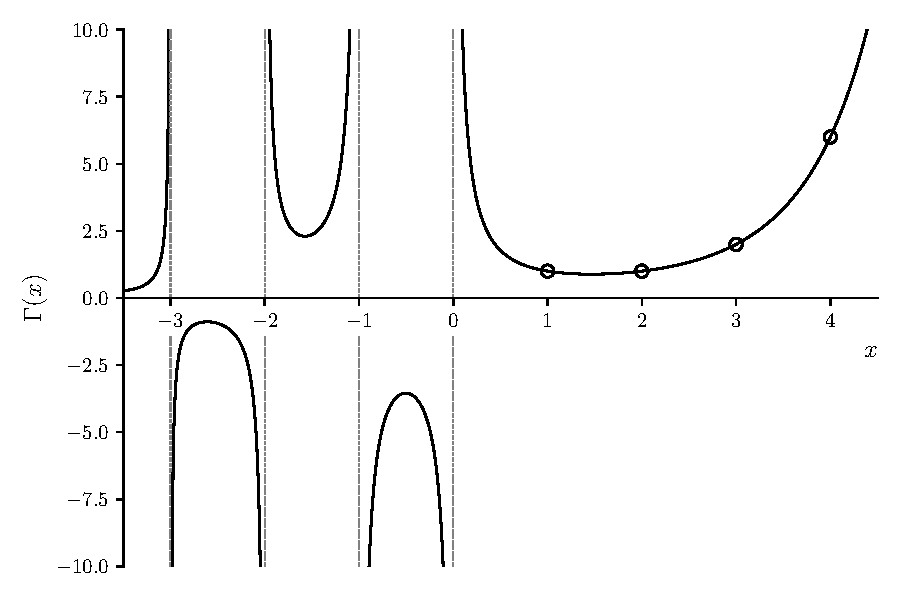
\includegraphics[width=\linewidth]{figs/gamma.pdf}
  \caption{The Gamma function, $\Gamma(x)$ on the real line. Open circles represent the value of $(x+1)!$, and dotted vertical lines are the poles at every non-positive integer.}
  \label{fig:gamma}
\end{figure}

Another useful formula is the values of the Gamma function at half-integers:
\begin{e}
  \Gamma\parens{z+\frac{1}{2}} = \frac{\sqrt{\pi}}{4^{z-\frac{1}{2}}}\frac{\Gamma(2z)}{\Gamma(z)}
\end{e}
which reduces to the special case of $\Gamma(\frac{1}{2}) = \sqrt{\pi}$. The Gamma function can also be used to aid in evaluating the following integral 
\begin{e}
  B(a,b) = \int_0^1 dt\, t^{a-1} (1-t)^{b-1}
  \label{eqn:beta-function}
\end{e}
which is called the \emphi{Beta function}. It appears in QFT as well as in probability and various trigonometric functions. It is related to the Gamma function via
\begin{e}
  B(a,b) = \frac{\Gamma(a)\Gamma(b)}{\Gamma(a+b)}.
  \label{eqn:beta-to-gamma}
\end{e}
Below, we use the Beta and Gamma functions to compute the surface area of a $d$-dimensional sphere.

\subsection{Surface Area of Spheres}
In physics, integrals over quantities which are rotationally symmetrical are very common. Such integrals can be separated into a radial part and an angular part, even in an arbitrary $d$-dimensional space, by integrating over $d$-dimensional spheres like so
\begin{e}
  \int d^d x\, f(|x|) = \parens{\int dr\, r^{d-1} f(r)}A_d
  \label{eqn:radial-integral}
\end{e}
where $A_d$ is the surface area of the $d$-dimensional unit sphere. For example, $A_3 = 4\pi$ and $A_2=2\pi$.

The task of this section is to find the surface area of this $d$-dimensional sphere as a function of $d$, which we will do via recursion. Suppose we know the area $A_{d-1}$. This knowledge allows us to separate the $d$ dimensions into one $\hat z$ axis and $d-1$ other axes, which together form a hyperplane $P$. Now we can think two-dimensionally in terms of the plane $P$ and $\hat z$. (Figure \ref{fig:sphere-surface-area})

\begin{figure}
  \centering
  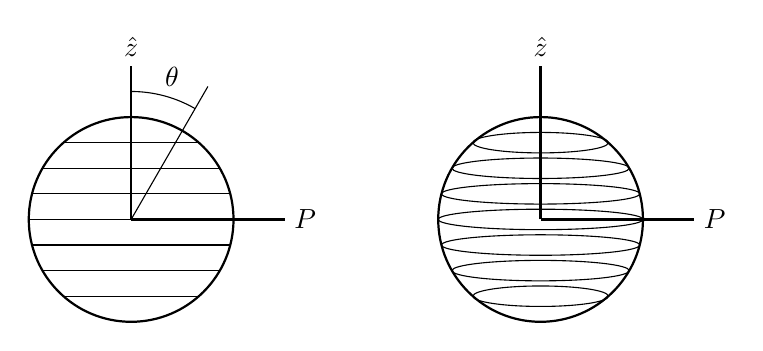
\begin{tikzpicture}[scale=1.3]
    \draw [thick] (-2,0) circle (1);
    \draw [thick] (-2,0) -- (-2,1.5);
    \draw [thick] (-2,0) -- (-0.5,0);
    \draw (-2,0) -- (-1.25,1.29903810567665);
    \draw (-2,1.25) arc (90:60:1.25);
    \draw (-1.6,1.2) node[anchor=south] {$\theta$};
    \draw (-2,1.5) node[anchor=south] {$\hat z$};
    \draw (-0.5,0) node[anchor=west] {$P$};
    \draw (-3,0) -- (-1,0);
    \draw (-2.968245836551854,0.25) -- (-1.0317541634481457,0.25);
    \draw (-2.8660254037844384,0.5) -- (-1.1339745962155614,0.5);
    \draw (-2.6614378277661475,0.75) -- (-1.3385621722338523,0.75);
    \draw (-2.968245836551854,-0.25) -- (-1.0317541634481457,-0.25);
    \draw (-2.8660254037844384,-0.5) -- (-1.1339745962155614,-0.5);
    \draw (-2.6614378277661475,-0.75) -- (-1.3385621722338523,-0.75);


    \draw [thick] (2,0) circle (1);
    \draw [thick] (2,0) -- (2,1.5);
    \draw [thick] (2,0) -- (3.5,0);
    \draw (2,1.5) node[anchor=south] {$\hat z$};
    \draw (3.5,0) node[anchor=west] {$P$};
    \draw (2, 0) ellipse (1 and 0.1);
    \draw (2, 0.25) ellipse (0.9682458365518543 and 0.1);
    \draw (2, 0.5) ellipse (0.8660254037844384 and 0.1);
    \draw (2, 0.75) ellipse (0.6614378277661475 and 0.1);
    \draw (2, -0.25) ellipse (0.9682458365518543 and 0.1);
    \draw (2, -0.5) ellipse (0.8660254037844384 and 0.1);
    \draw (2, -0.75) ellipse (0.6614378277661475 and 0.1);
  \end{tikzpicture}
  \caption{Stacking $d-1$-dimensional spheres to form a $d$-dimensional sphere for $d=3$.}
  \label{fig:sphere-surface-area}
\end{figure}

The $d$-sphere corresponds to many $d-1$-spheres stacked along the $\hat z$ axis, just as a normal three dimensional sphere is a stack of circles. As the stack grows, the circles (or $d-1$-spheres) shrink, following $r=\sin\theta$ as $\theta$ rises from $\pi/2$ on the equator to zero at the pole. The general scaling law of area with radius implies that the area also shrinks as $r^{d-2}$. To compute the area in $d$-space $dA$, we must also multiply by the thickness of each slice so that $dA = A_{d-1}\sin^{d-2}\theta d\theta$ to the total area per slice. Integrating this equation,
\begin{es}
  A_d &= A_{d-1}\int_0^\pi d\theta\,\sin^{d-2}\theta \\
  &= -A_{d-1}\int_0^\pi d(\cos\theta)\,\sin^{d-3}\theta\\
  &= A_{d-1}\int_{-1}^1 dx\,\parens{1-x^2}^{\frac{d-3}{2}}\\
  &= A_{d-1}\int_0^1 dt\,t^{-\frac{1}{2}}\parens{1-t}^{\frac{d-3}{2}}
  \label{eqn:sphere-area-working}
\end{es}
where in the second line we substituted variables from $\theta \rightarrow \cos\theta$, in the third line we expressed $\sin\theta = \sqrt{1-\cos^2\theta}$, and in the last line we substituted variables $x^2 \rightarrow t$. The last integral is the Beta function $B(\frac{1}{2}, \frac{d-1}{2})$ we defined in the previous section, so we may immediately write it in terms of $\Gamma$ functions:
\begin{e}
  A_d = A_{d-1} \frac{\Gamma\parens{\frac{1}{2}}\Gamma\parens{\frac{d-1}{2}}}{\Gamma\parens{\frac{d}{2}}} = A_{d-1} \sqrt{\pi}\frac{\Gamma\parens{\frac{d-1}{2}}}{\Gamma\parens{\frac{d}{2}}}.
\end{e}
Now we must turn the above recursive equation into a formula for $A_d$, but fortunately this is not difficult due to the $\Gamma$ function's own recursion relation (\ref{eqn:gamma-recursion}). The following formula checks out:
\begin{e}
  A_d = \frac{2\pi^{d/2}}{\Gamma\parens{\frac{d}{2}}}.
  \label{eqn:surface-area-sphere}
\end{e}


(\ref{eqn:surface-area-sphere}) draws a fascinating and unexpected connection between the Gamma function, which descended from factorials, and spheres. While it is possible to evaluate the first line (\ref{eqn:sphere-area-working}) without referring to the Gamma function if $d$ is an integer, our result is actually applicable for all $d$ because the Beta function is valid for any complex input. The validity of (\ref{eqn:surface-area-sphere}) for non-integers seems irrelevant, but it is actually critical in QFT and will be used in chapter \ref{chap:renormalization}.
